\documentclass[12pt]{article}

%***************************************************************************************************
% Math
\usepackage{fancyhdr} 
\usepackage{amsfonts}
\usepackage{amsmath}
\usepackage{amssymb}
\usepackage{amsthm}
%\usepackage{dsfont}

%***************************************************************************************************
% Macros
\usepackage{calc}

%***************************************************************************************************
% Commands and Custom Variables	
\newcommand{\problem}[1]{\hspace{-4 ex} \large \textbf{Problem #1} }
\let\oldemptyset\emptyset
\let\emptyset\varnothing
\newcommand{\norm}[1]{\left\lVert#1\right\rVert}
\newcommand{\sint}{\text{s}\kern-5pt\int}
\newcommand{\powerset}{\mathcal{P}}
\renewenvironment{proof}{\hspace{-4 ex} \emph{Proof}:}{\qed}

%***************************************************************************************************
%page
\usepackage[margin=1in]{geometry}
\usepackage{setspace}
%\doublespacing
\allowdisplaybreaks
\pagestyle{fancy}
\fancyhf{}
\rhead{Shaw \space \thepage}
\setlength\parindent{0pt}

%***************************************************************************************************
%Code
\usepackage{listings}
\usepackage{courier}
\lstset{
	language=Python,
	showstringspaces=false,
	formfeed=newpage,
	tabsize=4,
	commentstyle=\itshape,
	basicstyle=\ttfamily,
}

%***************************************************************************************************
%Images
\usepackage{graphicx}
\graphicspath{ {images/} }
\usepackage{float}

%tikz
\usepackage[utf8]{inputenc}
\usepackage{pgfplots}
\usepgfplotslibrary{groupplots}

%***************************************************************************************************
%Hyperlinks
%\usepackage{hyperref}
%\hypersetup{
%	colorlinks=true,
%	linkcolor=blue,
%	filecolor=magenta,      
%	urlcolor=cyan,
%}


\begin{document}
	\thispagestyle{empty}
	
	\begin{flushright}
		Sage Shaw \\
		m565 - Fall 2017 \\
		\today
	\end{flushright}
	
{\large \textbf{HW 4}}\bigbreak

%***************************************************************************************************
\singlespacing
\problem{1} We write Lagrange's interpolation formula as 
$$ \sum\limits_{j=0}^n l_j(x)f(x_j)  $$
Show that 
\begin{align}
	\sum\limits_{j=0}^n l_j(x)x_j \equiv x
\end{align}
	
	\doublespacing
	\begin{proof}
		Consider the function $f(x)=x$. Given the sample points $\{x_j\}_{0=j}^n$, $f(x_j)=x_j$. Since $f$ is a polynomial, it is the polynomial that interpolates the points $\Big \{ \big(x_j,f(x_j) \big) \Big\}_{0=j}^n$ and thus
		$$ \sum\limits_{j=0}^n l_j(x)x_j = \sum\limits_{j=0}^n l_j(x)f(x_j) = f(x) = x$$
	\end{proof}


%***************************************************************************************************
\singlespacing
\problem{2} Let $$E_1(x) = \int_{x}^{\infty}\frac{e^{-t}}{t}dt \ \ x>0$$ 
We would like to construct a table of values over the interval $x \in [1,10]$ such that the second degree polynomial interpolation between any three adjacent points in the table will give an error less than or equal to $10^{-8}$.

	We will use the error formula
	$$
	\vert P_2(x) - f(x) \vert \leq \frac{\vert (x-x_0)(x-x_1)(x-x_2) \vert}{3!} \max_{a\leq x \leq b} \big\vert f^{(3)}(x) \big\vert
	$$
	First we will find the maximum of the third derivative over $1 \leq x \leq 10$.
	\begin{align*}
		f^{\prime}(x) & = \frac{d}{dx} \int_{x}^{\infty}\frac{e^{-t}}{t}dt \\
		& = \frac{d}{dx} -\int_{\infty}^{x}\frac{e^{-t}}{t}dt \\
		& = -\frac{e^{-x}}{x} \\
		& = -x^{-1}e^{-x} \\
		f^{\prime\prime}(x) & = \frac{d}{dx} -x^{-1}e^{-x} \\
		& = x^{-2} e^{-x} + x^{-1}e^{-x} \\
		f^{(3)}(x) & = \frac{d}{dx} (x^{-2} e^{-x} + x^{-1}e^{-x}) \\
		& = -2x^{-3}e^{-x} - x^{-2} e^{-x} - x^{-2} e^{-x} - x^{-1}e^{-x} \\
		& = -2x^{-3}e^{-x} - 2x^{-2} e^{-x} - x^{-1}e^{-x} \\
		& = (-2x^{-3} - 2x^{-2} - x^{-1}) e^{-x}
	\end{align*}
	This function has no local extrema except at the end points. It is clear that the maximum value of the absolute value of the third derivative is at $x=1$, thus $\max_{1\leq x \leq 10} \big\vert f^{(3)}(x) \big\vert = \tfrac{5}{e}$. \bigbreak
	
	Next we will find the maximum value of $\vert (x-x_0)(x-x_1)(x-x_2) \vert$ over our interval. Note that if $x$ is one of our data points, this product is zero. Without loss of generality we can assume that $x_0 < x < x_1$ for some ordered points $x_0 < x_1 < x_2$. Since all of our points are equally spaced, $\vert x_0 - x_1 \vert = \vert x_1 - x_2 \vert = h$ where $h$ is the step size in our table. Letting $ x-x_0 = w$ we have the following substitutions $ x_1-x = h-w, x_2 - x = 2h - w$. Now our problem is to find the maximum value of $ w(w-h)(w-2h)$ for $ 0 \leq w \leq h$. Note that each term is positive so we may drop the absolute. Distributing we have $w^3 - 3w^2h + 2wh^2$. To maximize this we find the root of the derivative $3w^2 + 6wh + 2h^2$. Applying the quadratic formula we find that our function has a maximum at 
	$$
	w = \frac{-6h \pm \sqrt{(6h)^2 - 4(3)(2h^2)}}{2(3)} = h \frac{3-\sqrt{3}}{3}
	$$
	Substituting this back in we have the maximum value
	$$
	(h \tfrac{3-\sqrt{3}}{3})^3 - 3(h \tfrac{3-\sqrt{3}}{3})^2h + 2(h \tfrac{3-\sqrt{3}}{3})h^2 = \frac{2 \sqrt{3}}{9}h^3
	$$
	Finally we get that our error is bounded by
	$$
	\vert P_2(x) - f(x) \vert \leq \frac{5\sqrt{3}}{27e}h^3
	$$
	If we would like our error to be below $10^{-8}$ we simplify $\frac{5\sqrt{3}}{27e}h^3 < 10^{-8}$ to obtain a maximum step size
	$$
	h < \sqrt[3]{\frac{27e10^{-8}}{5 \sqrt{3}}} \approx 0.00439
	$$
	
%***************************************************************************************************
\singlespacing
\problem{3}

%***************************************************************************************************
\problem{4 (a)} Create a program for interpolating data using the the barycentric formula.

	\begin{lstlisting}
def polyinterp(u, x, y, w=None):
	if w == None:
		w = baryweights(x)
	ret = np.zeros(len(u))
	for i in range(len(ret)):
		if u[i] in x:
			ret[i] = y[np.where(x==u[i])]
		else:
			weights = w /(u[i] - x)
			ret[i] = weights.dot(y)/sum(weights)
	return ret

def baryweights(x):
	w = np.ones(len(x))
	for j, xj in enumerate(x):
		for xi in x[np.arange(len(x))!=j]: 
			w[j] /= (xj - xi)
	return w
	\end{lstlisting}

%***************************************************************************************************
\problem{4 (b)} Using equispaced points, the Chebyshev points of the first and second kind, and Legendre points, interpolate $f(x) = \sqrt{x^2 +.1}$ using 15 points. Evaluate it at 201 equally spaced points on the interval $[-1,1]$, and plot the error. Decide which point set produces the best result?

	\begin{lstlisting}
def p4b():
	samples = []
	labels = []
	x = np.linspace(-1,1,15)
	samples.append(x)
	labels.append('Equispaced points:')
	x = []
	for j in range(0,15):
		x.append( -1* np.cos( (2*j+1)/29 * np.pi))
	samples.append(np.array(x))
	labels.append('First kind Chebyshev points:')
	x = []
	for j in range(0,15):
		x.append( -1* np.cos( (j*np.pi)/14 ) )
	samples.append(np.array(x))
	labels.append('Second kind Chebyshev points:')
	x = [-0.987992518020485,
			-0.394151347077563,
			0.570972172608539,
			-0.937273392400706,
			-0.201194093997435,
			0.724417731360170,
			-0.848206583410427,
			0,
			0.848206583410427,
			-0.724417731360170,
			0.201194093997435,
			0.937273392400706,
			-0.570972172608539,
			0.394151347077563,
			0.987992518020485]
	samples.append(np.array(x))
	labels.append('Legendre points:')
	for x, l in zip(samples, labels):
		y = p4_foo(x)
		u = np.linspace(-1,1,201)
		p = polyinterp(u, x, y)
		f = p4_foo(u)
		print(l)
		print('Eucidian norm: %f' % np.linalg.norm(f-p))
		print('Infinity norm: %f' % np.linalg.norm(f-p,np.inf))
		plt.subplot(2,1,1)
		plt.plot(u,p, 'r-')
		plt.plot(u,f, 'k-')
		plt.plot(x,y, 'bo')
		plt.xlim( (-1, 1) )
		plt.ylim( (.2, 1.2) )
		
		plt.subplot(2,1,2)
		plt.plot(u, p-f, 'k-')
		plt.xlim( (-1, 1) )
		y_range = np.max( np.abs(p-f) )
		plt.ylim( (-y_range, y_range) )
		plt.show()
	\end{lstlisting}
	
	The code above gives the following output.
	\begin{lstlisting}
Equispaced points:
Eucidian norm: 0.084877
Infinity norm: 0.024440
First kind Chebyshev points:
Eucidian norm: 0.001919
Infinity norm: 0.000347
Second kind Chebyshev points:
Eucidian norm: 0.001945
Infinity norm: 0.000266
Legendre points:
Eucidian norm: 0.001945
Infinity norm: 0.000621
	\end{lstlisting}
	
	\begin{figure}[H]
		\caption{Equispaced points}
		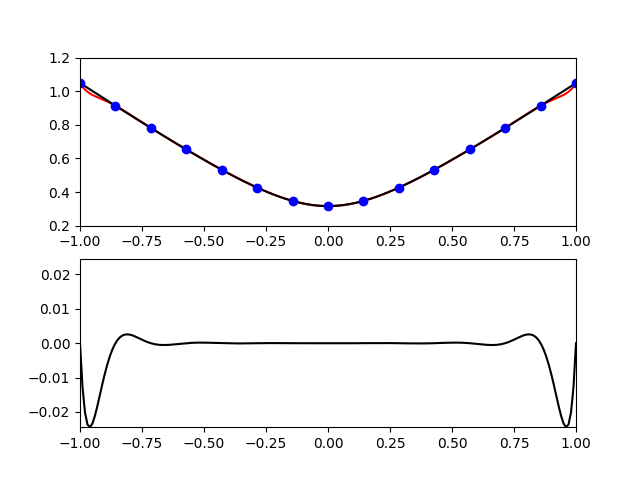
\includegraphics[width=0.80\textwidth]{hw4_figure_1}
		\centering
	\end{figure}
	\begin{figure}[H]
		\caption{First kind Chebyshev points}
		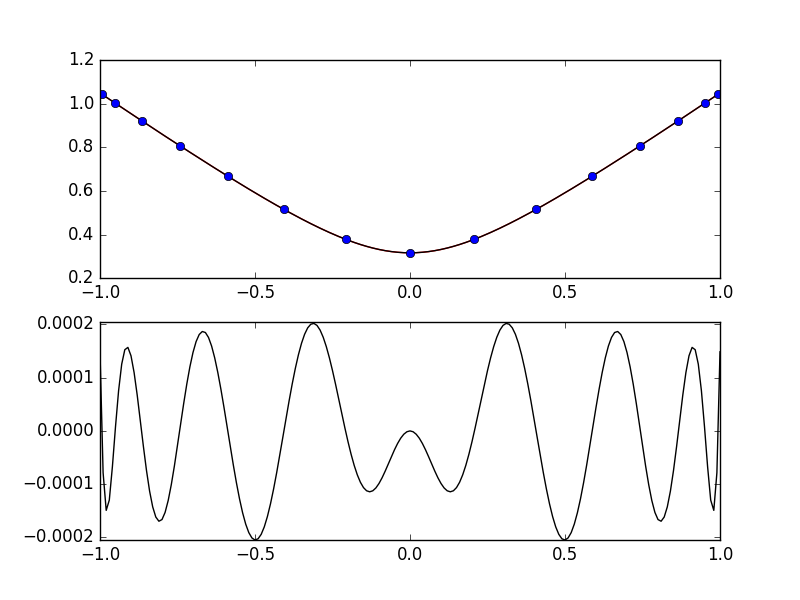
\includegraphics[width=0.80\textwidth]{hw4_figure_2}
		\centering
	\end{figure}
	\begin{figure}[H]
		\caption{Second kind Chebyshev points}
		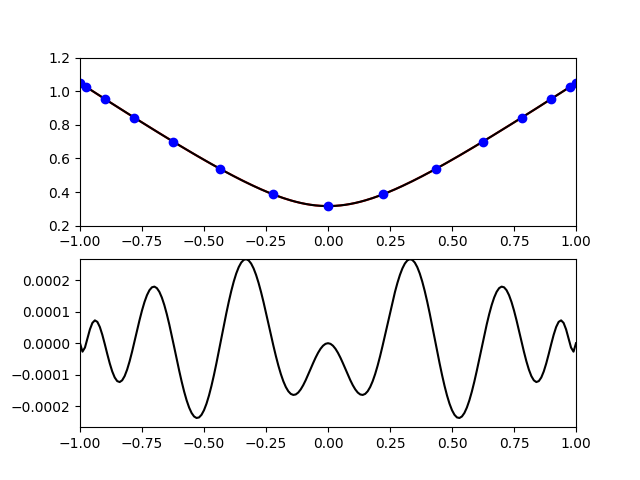
\includegraphics[width=0.80\textwidth]{hw4_figure_3}
		\centering
	\end{figure}
	\begin{figure}[H]
		\caption{Legendre points}
		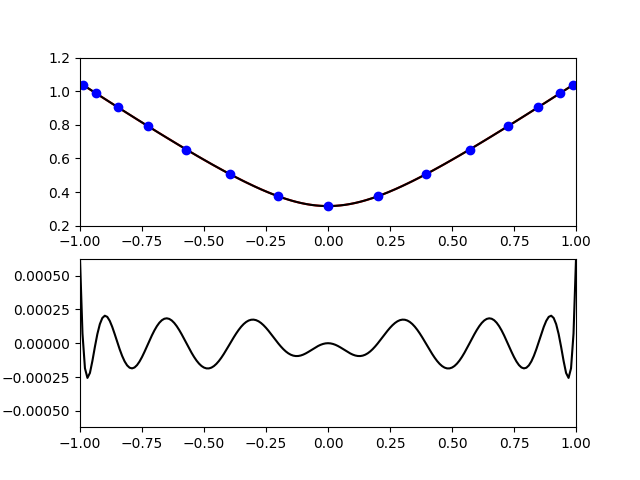
\includegraphics[width=0.80\textwidth]{hw4_figure_4}
		\centering
	\end{figure}
%	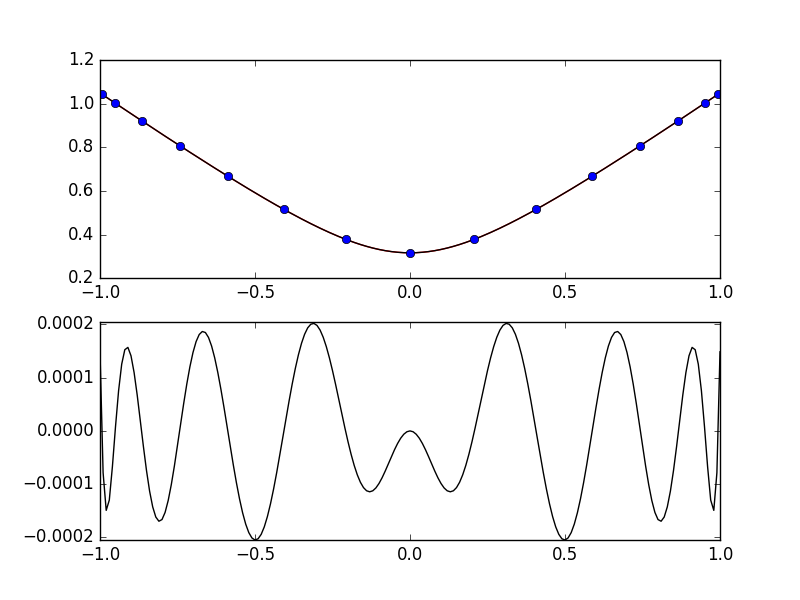
\includegraphics[width=0.85\textwidth]{hw4_figure_2} \\
%	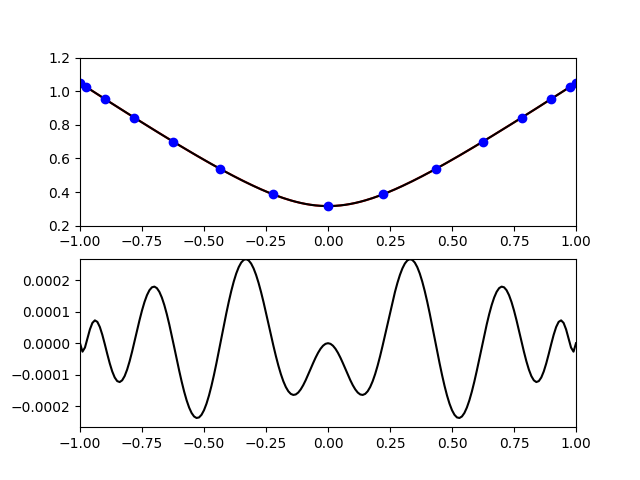
\includegraphics[width=.85\textwidth]{hw4_figure_3} \\
%	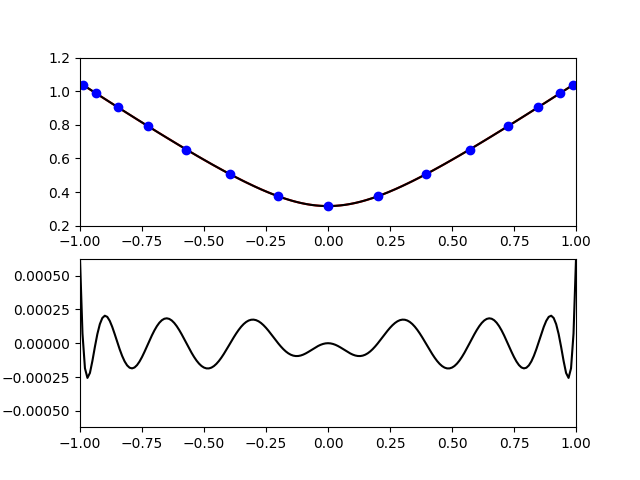
\includegraphics[width=.85\textwidth]{hw4_figure_4} \\
%	%% This file was created by matplotlib2tikz v0.6.13.
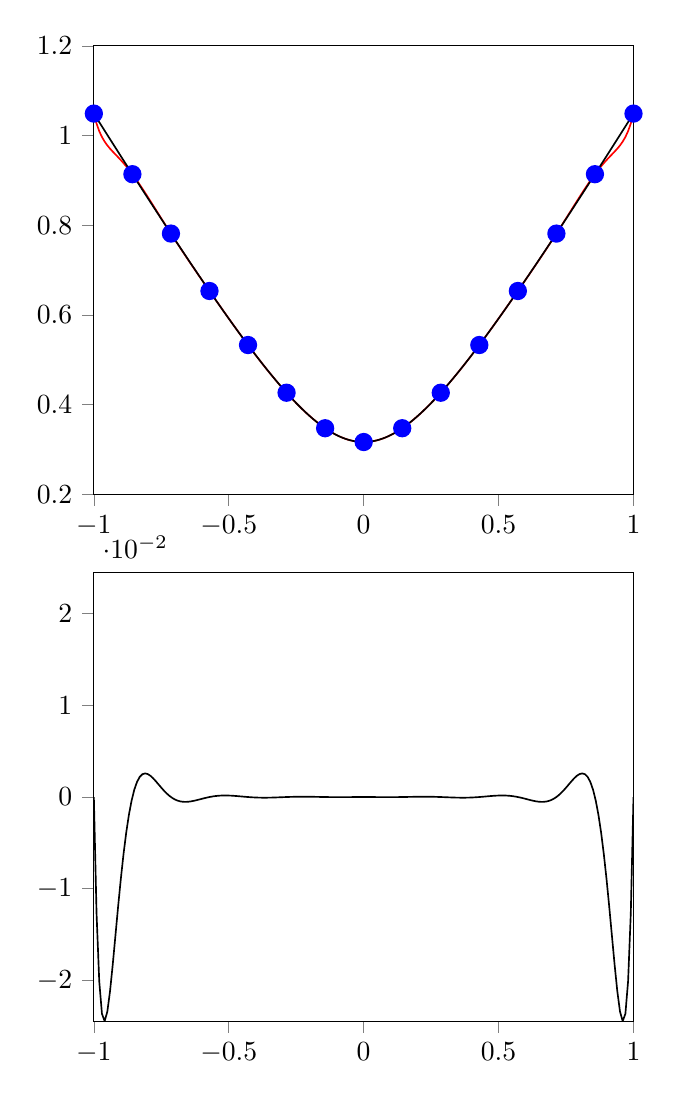
\begin{tikzpicture}

\begin{groupplot}[group style={group size=1 by 2}]
\nextgroupplot[
xmin=-1, xmax=1,
ymin=0.2, ymax=1.2,
tick align=outside,
tick pos=left,
x grid style={lightgray!92.026143790849673!black},
y grid style={lightgray!92.026143790849673!black}
]
\addplot [semithick, red, forget plot]
table {%
-1 1.04880884817015
-0.99 1.02659991313634
-0.98 1.00967258211117
-0.97 0.996614026716382
-0.96 0.986302184269025
-0.95 0.977857316353005
-0.94 0.970600230842617
-0.93 0.964016407207195
-0.92 0.957725336497917
-0.91 0.951454453499305
-0.9 0.945017099455632
-0.89 0.938294009874922
-0.88 0.931217873476089
-0.87 0.923760555667185
-0.86 0.915922623300696
-0.85 0.907724847107188
-0.84 0.899201394410172
-0.83 0.890394457708803
-0.82 0.881350094704801
-0.81 0.872115082557669
-0.8 0.862734613778574
-0.79 0.853250683407881
-0.78 0.843701037143277
-0.77 0.834118568064181
-0.76 0.824531065692751
-0.75 0.814961235492768
-0.74 0.805426919675971
-0.73 0.795941461493997
-0.72 0.786514165167359
-0.71 0.777150812357636
-0.7 0.767854203734625
-0.69 0.758624700828598
-0.68 0.749460749084525
-0.67 0.740359367938815
-0.66 0.731316597902627
-0.65 0.722327898135703
-0.64 0.713388490902193
-0.63 0.704493651680964
-0.62 0.695638945618015
-0.61 0.686820412514039
-0.6 0.678034703687167
-0.59 0.669279174886707
-0.58 0.6605519400014
-0.57 0.651851890644508
-0.56 0.643178686843734
-0.55 0.63453272404871
-0.54 0.625915081521762
-0.53 0.617327456924947
-0.52 0.608772091581272
-0.51 0.600251690491277
-0.5 0.591769340746087
-0.49 0.583328431510587
-0.48 0.574932578269536
-0.47 0.566585553547109
-0.46 0.558291225836819
-0.45 0.550053508022478
-0.44 0.541876316138889
-0.43 0.533763538918905
-0.42 0.525719018205844
-0.41 0.517746539980071
-0.4 0.509849835458258
-0.39 0.50203259147463
-0.38 0.494298469145788
-0.37 0.486651129654442
-0.36 0.479094265861492
-0.35 0.471631638369085
-0.34 0.464267114607588
-0.33 0.457004709504633
-0.32 0.449848626311811
-0.31 0.442803296211466
-0.3 0.435873415399241
-0.29 0.429063978434347
-0.28 0.422380306765778
-0.27 0.415828071475393
-0.26 0.409413309424795
-0.25 0.403142432148814
-0.24 0.397022227001081
-0.23 0.391059850223459
-0.22 0.385262811778135
-0.21 0.379638951946125
-0.2 0.374196409856207
-0.19 0.368943584261529
-0.18 0.363889087025128
-0.17 0.359041689908429
-0.16 0.35441026537673
-0.15 0.350003722241376
-0.14 0.345830937048439
-0.13 0.341900682197457
-0.12 0.33822155183038
-0.11 0.334801886569902
-0.1 0.331649698207664
-0.09 0.32877259544644
-0.08 0.326177711786635
-0.07 0.323871636616782
-0.0599999999999999 0.321860350520894
-0.0499999999999999 0.320149165753446
-0.04 0.318742672756554
-0.03 0.317644693504774
-0.02 0.316858242362343
-0.01 0.316385495027148
0 0.316227766016838
0.01 0.316385495027147
0.02 0.316858242362343
0.03 0.317644693504774
0.04 0.318742672756555
0.05 0.320149165753446
0.0600000000000001 0.321860350520894
0.0700000000000001 0.323871636616782
0.0800000000000001 0.326177711786635
0.0900000000000001 0.32877259544644
0.1 0.331649698207664
0.11 0.334801886569902
0.12 0.33822155183038
0.13 0.341900682197457
0.14 0.345830937048439
0.15 0.350003722241376
0.16 0.35441026537673
0.17 0.359041689908429
0.18 0.363889087025128
0.19 0.368943584261529
0.2 0.374196409856207
0.21 0.379638951946125
0.22 0.385262811778134
0.23 0.391059850223459
0.24 0.397022227001082
0.25 0.403142432148814
0.26 0.409413309424795
0.27 0.415828071475393
0.28 0.422380306765778
0.29 0.429063978434347
0.3 0.435873415399241
0.31 0.442803296211467
0.32 0.449848626311811
0.33 0.457004709504633
0.34 0.464267114607588
0.35 0.471631638369085
0.36 0.479094265861492
0.37 0.486651129654442
0.38 0.494298469145788
0.39 0.50203259147463
0.4 0.509849835458258
0.41 0.51774653998007
0.42 0.525719018205845
0.43 0.533763538918905
0.44 0.541876316138889
0.45 0.550053508022479
0.46 0.558291225836819
0.47 0.566585553547109
0.48 0.574932578269536
0.49 0.583328431510587
0.5 0.591769340746087
0.51 0.600251690491277
0.52 0.608772091581272
0.53 0.617327456924947
0.54 0.625915081521762
0.55 0.63453272404871
0.56 0.643178686843734
0.57 0.651851890644508
0.58 0.6605519400014
0.59 0.669279174886707
0.6 0.678034703687167
0.61 0.686820412514039
0.62 0.695638945618015
0.63 0.704493651680964
0.64 0.713388490902193
0.65 0.722327898135703
0.66 0.731316597902627
0.67 0.740359367938815
0.68 0.749460749084525
0.69 0.758624700828598
0.7 0.767854203734624
0.71 0.777150812357636
0.72 0.786514165167359
0.73 0.795941461493997
0.74 0.805426919675971
0.75 0.814961235492768
0.76 0.824531065692751
0.77 0.834118568064181
0.78 0.843701037143278
0.79 0.853250683407881
0.8 0.862734613778574
0.81 0.872115082557668
0.82 0.881350094704802
0.83 0.890394457708804
0.84 0.899201394410173
0.85 0.907724847107189
0.86 0.915922623300696
0.87 0.923760555667185
0.88 0.931217873476087
0.89 0.938294009874922
0.9 0.94501709945563
0.91 0.951454453499302
0.92 0.957725336497916
0.93 0.964016407207187
0.94 0.970600230842614
0.95 0.977857316353002
0.96 0.986302184269022
0.97 0.996614026716374
0.98 1.00967258211117
0.99 1.02659991313634
1 1.04880884817015
};
\addplot [semithick, black, forget plot]
table {%
-1 1.04880884817015
-0.99 1.03927859595009
-0.98 1.02975725294848
-0.97 1.02024506859872
-0.96 1.01074230147946
-0.95 1.00124921972504
-0.94 0.991766101457395
-0.93 0.982293235240883
-0.92 0.972830920561225
-0.91 0.963379468330107
-0.9 0.953939201416946
-0.89 0.94451045520947
-0.88 0.935093578204877
-0.87 0.92568893263342
-0.86 0.916296895116425
-0.85 0.906917857360853
-0.84 0.897552226892675
-0.83 0.888200427831466
-0.82 0.878862901708793
-0.81 0.869540108333135
-0.8 0.860232526704263
-0.79 0.850940655980192
-0.78 0.841665016500033
-0.77 0.83240615086627
-0.76 0.823164625090267
-0.75 0.813941029804985
-0.74 0.804735981549228
-0.73 0.795550124127952
-0.72 0.7863841300535
-0.71 0.777238702072922
-0.7 0.768114574786861
-0.69 0.759012516365837
-0.68 0.749933330370107
-0.67 0.740877857679658
-0.66 0.731846978541279
-0.65 0.722841614740048
-0.64 0.71386273190299
-0.63 0.704911341943084
-0.62 0.695988505652213
-0.61 0.687095335452075
-0.6 0.678232998312527
-0.59 0.669402718847182
-0.58 0.66060578259655
-0.57 0.651843539509291
-0.56 0.643117407632541
-0.55 0.634428877022476
-0.54 0.625779513886481
-0.53 0.617170964968379
-0.52 0.608604962188118
-0.51 0.6000833275471
-0.5 0.591607978309962
-0.49 0.583180932472933
-0.48 0.574804314527997
-0.47 0.566480361530742
-0.46 0.558211429478115
-0.45 0.55
-0.44 0.541848687365763
-0.43 0.533760245803301
-0.42 0.525737577123797
-0.41 0.517783738639985
-0.4 0.509901951359279
-0.39 0.502095608425328
-0.38 0.494368283772331
-0.37 0.486723740945518
-0.36 0.479165942028438
-0.35 0.47169905660283
-0.34 0.464327470649756
-0.33 0.457055795281058
-0.32 0.44988887516808
-0.31 0.442831796509691
-0.3 0.435889894354067
-0.29 0.429068759058499
-0.28 0.422374241638858
-0.27 0.415812457725836
-0.26 0.409389789809174
-0.25 0.403112887414928
-0.24 0.396988664825584
-0.23 0.391024295920343
-0.22 0.385227205685164
-0.21 0.379605057922046
-0.2 0.374165738677394
-0.19 0.368917334913934
-0.18 0.363868107973205
-0.17 0.359026461420325
-0.16 0.354400902933387
-0.15 0.35
-0.14 0.345832329315812
-0.13 0.341906419945575
-0.12 0.338230690505755
-0.11 0.334813380855664
-0.1 0.33166247903554
-0.09 0.328785644455472
-0.08 0.326190128606002
-0.07 0.323882694814033
-0.0599999999999999 0.321869538788622
-0.0499999999999999 0.320156211871642
-0.04 0.318747549010185
-0.03 0.317647603485372
-0.02 0.316859590355097
-0.01 0.316385840391127
0 0.316227766016838
0.01 0.316385840391127
0.02 0.316859590355097
0.03 0.317647603485372
0.04 0.318747549010185
0.05 0.320156211871642
0.0600000000000001 0.321869538788622
0.0700000000000001 0.323882694814033
0.0800000000000001 0.326190128606002
0.0900000000000001 0.328785644455472
0.1 0.33166247903554
0.11 0.334813380855664
0.12 0.338230690505755
0.13 0.341906419945575
0.14 0.345832329315812
0.15 0.35
0.16 0.354400902933387
0.17 0.359026461420325
0.18 0.363868107973205
0.19 0.368917334913934
0.2 0.374165738677394
0.21 0.379605057922046
0.22 0.385227205685164
0.23 0.391024295920343
0.24 0.396988664825584
0.25 0.403112887414928
0.26 0.409389789809174
0.27 0.415812457725836
0.28 0.422374241638858
0.29 0.429068759058499
0.3 0.435889894354067
0.31 0.442831796509691
0.32 0.44988887516808
0.33 0.457055795281058
0.34 0.464327470649756
0.35 0.47169905660283
0.36 0.479165942028438
0.37 0.486723740945518
0.38 0.494368283772331
0.39 0.502095608425328
0.4 0.509901951359279
0.41 0.517783738639985
0.42 0.525737577123797
0.43 0.533760245803301
0.44 0.541848687365763
0.45 0.55
0.46 0.558211429478115
0.47 0.566480361530742
0.48 0.574804314527997
0.49 0.583180932472933
0.5 0.591607978309962
0.51 0.6000833275471
0.52 0.608604962188118
0.53 0.617170964968379
0.54 0.625779513886481
0.55 0.634428877022476
0.56 0.643117407632541
0.57 0.651843539509291
0.58 0.66060578259655
0.59 0.669402718847182
0.6 0.678232998312527
0.61 0.687095335452075
0.62 0.695988505652213
0.63 0.704911341943084
0.64 0.71386273190299
0.65 0.722841614740048
0.66 0.73184697854128
0.67 0.740877857679658
0.68 0.749933330370107
0.69 0.759012516365837
0.7 0.768114574786861
0.71 0.777238702072922
0.72 0.7863841300535
0.73 0.795550124127952
0.74 0.804735981549228
0.75 0.813941029804985
0.76 0.823164625090267
0.77 0.83240615086627
0.78 0.841665016500033
0.79 0.850940655980192
0.8 0.860232526704263
0.81 0.869540108333135
0.82 0.878862901708793
0.83 0.888200427831466
0.84 0.897552226892675
0.85 0.906917857360853
0.86 0.916296895116425
0.87 0.92568893263342
0.88 0.935093578204877
0.89 0.94451045520947
0.9 0.953939201416946
0.91 0.963379468330107
0.92 0.972830920561225
0.93 0.982293235240883
0.94 0.991766101457395
0.95 1.00124921972504
0.96 1.01074230147946
0.97 1.02024506859872
0.98 1.02975725294848
0.99 1.03927859595009
1 1.04880884817015
};
\addplot [semithick, blue, mark=*, mark size=3, mark options={solid}, only marks, forget plot]
table {%
-1 1.04880884817015
-0.857142857142857 0.913615826018256
-0.714285714285714 0.781155606542418
-0.571428571428571 0.653093111466426
-0.428571428571429 0.532610053780207
-0.285714285714286 0.426183825433609
-0.142857142857143 0.346998794328318
0 0.316227766016838
0.142857142857143 0.346998794328318
0.285714285714286 0.426183825433608
0.428571428571428 0.532610053780207
0.571428571428571 0.653093111466426
0.714285714285714 0.781155606542418
0.857142857142857 0.913615826018256
1 1.04880884817015
};
\nextgroupplot[
xmin=-1, xmax=1,
ymin=-0.0244401172104404, ymax=0.0244401172104404,
tick align=outside,
tick pos=left,
x grid style={lightgray!92.026143790849673!black},
y grid style={lightgray!92.026143790849673!black}
]
\addplot [semithick, black, forget plot]
table {%
-1 0
-0.99 -0.0126786828137544
-0.98 -0.0200846708373055
-0.97 -0.0236310418823347
-0.96 -0.0244401172104374
-0.95 -0.0233919033720339
-0.94 -0.0211658706147781
-0.93 -0.0182768280336878
-0.92 -0.0151055840633074
-0.91 -0.0119250148308022
-0.9 -0.00892210196131371
-0.89 -0.00621644533454835
-0.88 -0.00387570472878818
-0.87 -0.00192837696623527
-0.86 -0.000374271815728244
-0.85 0.000806989746335862
-0.84 0.00164916751749677
-0.83 0.00219402987733697
-0.82 0.00248719299600775
-0.81 0.00257497422453379
-0.8 0.00250208707431088
-0.79 0.0023100274276886
-0.78 0.0020360206432446
-0.77 0.00171241719791049
-0.76 0.0013664406024837
-0.75 0.00102020568778294
-0.74 0.000690938126742813
-0.73 0.000391337366045352
-0.72 0.000130035113858895
-0.71 -8.78897152853941e-05
-0.7 -0.000260371052236308
-0.69 -0.000387815537238989
-0.68 -0.00047258128558203
-0.67 -0.000518489740843342
-0.66 -0.000530380638652184
-0.65 -0.000513716604345293
-0.64 -0.000474241000796849
-0.63 -0.000417690262120018
-0.62 -0.000349560034197838
-0.61 -0.000274922938035882
-0.6 -0.000198294625359474
-0.59 -0.000123543960475536
-0.58 -5.38425951502886e-05
-0.57 8.3511352170218e-06
-0.56 6.12792111928107e-05
-0.55 0.000103847026234227
-0.54 0.00013556763528122
-0.53 0.000156491956568194
-0.52 0.000167129393154553
-0.51 0.000168362944177436
-0.5 0.000161362436125301
-0.49 0.000147499037653986
-0.48 0.000128263741539625
-0.47 0.000105192016367051
-0.46 7.97963587041428e-05
-0.45 5.35080224783879e-05
-0.44 2.76287731261204e-05
-0.43 3.2931156042082e-06
-0.42 -1.85589179522161e-05
-0.41 -3.71986599139174e-05
-0.4 -5.21159010206107e-05
-0.39 -6.30169506975475e-05
-0.38 -6.9814626543041e-05
-0.37 -7.26112910762744e-05
-0.36 -7.16761669452559e-05
-0.35 -6.74182337452867e-05
-0.34 -6.0356042168197e-05
-0.33 -5.108577642432e-05
-0.32 -4.02488562683545e-05
-0.31 -2.85002982240989e-05
-0.3 -1.64789548265931e-05
-0.29 -4.78062415221192e-06
-0.28 6.06512692002958e-06
-0.27 1.56137495572195e-05
-0.26 2.35196156204154e-05
-0.25 2.95447338866106e-05
-0.24 3.35621754972704e-05
-0.23 3.55543031158589e-05
-0.22 3.56060929700974e-05
-0.21 3.38940240786623e-05
-0.2 3.06711788128911e-05
-0.19 2.62493475946535e-05
-0.18 2.09790519233866e-05
-0.17 1.52284881041465e-05
-0.16 9.36244334270864e-06
-0.15 3.72224137623611e-06
-0.14 -1.39226737244647e-06
-0.13 -5.73774811818417e-06
-0.12 -9.13867537538637e-06
-0.11 -1.14942857621925e-05
-0.1 -1.27808278755914e-05
-0.09 -1.30490090317625e-05
-0.08 -1.24168193671448e-05
-0.07 -1.10581972511126e-05
-0.0599999999999999 -9.18826772805525e-06
-0.0499999999999999 -7.04611819674072e-06
-0.04 -4.8762536300484e-06
-0.03 -2.9099805975985e-06
-0.02 -1.34799275386399e-06
-0.01 -3.45363979969981e-07
0 0
0.01 -3.45363980025493e-07
0.02 -1.34799275397501e-06
0.03 -2.90998059765402e-06
0.04 -4.87625362999289e-06
0.05 -7.04611819668521e-06
0.0600000000000001 -9.18826772799974e-06
0.0700000000000001 -1.10581972512236e-05
0.0800000000000001 -1.24168193672558e-05
0.0900000000000001 -1.3049009031818e-05
0.1 -1.27808278755359e-05
0.11 -1.14942857619704e-05
0.12 -9.13867537533086e-06
0.13 -5.73774811829519e-06
0.14 -1.39226737250198e-06
0.15 3.72224137612509e-06
0.16 9.36244334276415e-06
0.17 1.52284881041465e-05
0.18 2.09790519233866e-05
0.19 2.62493475944314e-05
0.2 3.06711788130576e-05
0.21 3.38940240786623e-05
0.22 3.56060929700419e-05
0.23 3.55543031158589e-05
0.24 3.35621754973814e-05
0.25 2.95447338866106e-05
0.26 2.35196156204154e-05
0.27 1.5613749557164e-05
0.28 6.06512692019612e-06
0.29 -4.7806241521009e-06
0.3 -1.64789548266486e-05
0.31 -2.85002982238214e-05
0.32 -4.02488562683545e-05
0.33 -5.10857764241535e-05
0.34 -6.0356042168086e-05
0.35 -6.74182337456752e-05
0.36 -7.1676166945478e-05
0.37 -7.26112910764964e-05
0.38 -6.9814626543041e-05
0.39 -6.30169506974365e-05
0.4 -5.21159010207217e-05
0.41 -3.71986599142504e-05
0.42 -1.85589179521051e-05
0.43 3.2931156042082e-06
0.44 2.76287731261204e-05
0.45 5.3508022478499e-05
0.46 7.97963587042538e-05
0.47 0.000105192016367273
0.48 0.000128263741539736
0.49 0.000147499037653875
0.5 0.000161362436125079
0.51 0.000168362944177436
0.52 0.000167129393154553
0.53 0.000156491956568305
0.54 0.00013556763528122
0.55 0.000103847026234116
0.56 6.12792111930327e-05
0.57 8.35113521713282e-06
0.58 -5.38425951501775e-05
0.59 -0.000123543960475314
0.6 -0.000198294625359585
0.61 -0.000274922938035993
0.62 -0.000349560034197727
0.63 -0.000417690262120018
0.64 -0.00047424100079696
0.65 -0.000513716604345404
0.66 -0.000530380638652517
0.67 -0.000518489740843786
0.68 -0.000472581285581808
0.69 -0.000387815537238989
0.7 -0.000260371052236641
0.71 -8.78897152855052e-05
0.72 0.000130035113858895
0.73 0.000391337366045463
0.74 0.000690938126742813
0.75 0.00102020568778305
0.76 0.00136644060248425
0.77 0.00171241719791093
0.78 0.00203602064324526
0.79 0.00231002742768827
0.8 0.00250208707431165
0.81 0.00257497422453346
0.82 0.0024871929960083
0.83 0.00219402987733763
0.84 0.00164916751749744
0.85 0.000806989746335973
0.86 -0.000374271815728688
0.87 -0.00192837696623482
0.88 -0.00387570472878951
0.89 -0.00621644533454824
0.9 -0.00892210196131582
0.91 -0.0119250148308049
0.92 -0.0151055840633086
0.93 -0.0182768280336957
0.94 -0.0211658706147813
0.95 -0.0233919033720378
0.96 -0.0244401172104404
0.97 -0.0236310418823422
0.98 -0.0200846708373057
0.99 -0.0126786828137586
1 0
};
\end{groupplot}

\end{tikzpicture}

	In each of the four figures the top subplot has the function $f(x) = \sqrt{x^2 + .1}$  in black, along with the interpolating polynomial in red, and the sample points in blue. The bottom subplot has the difference between the function and the interpolating polynomial. Note that the interpolating polynomial is so close to the function in figures 2-3 that it is not visible. \bigbreak
	
	Based off of the 2-norm and the $\infty$-norm any of these pointsets other than the equispaced very closely approximates our function. The Chebyshev points of the first kind minimize the 2-norm, and the Chebyshev points of the second kind minimize the infinity norm. It should be noted that from the graph of the error when choosing the Legendre points, we can see that the error is smaller than both kinds of Chebyshev points when not near the ends of the interval. One might gather that the Legendre points are the best choice when our function need not be evaluated near the end points. \bigbreak
	
%***************************************************************************************************
\problem{4 (c)} Show that for equally spaced points between $[-1,1]$, that 
$$
w_j = \frac{ (\tfrac{n}{2})^n (-1)^{n-j} }{ n! }  {{n}\choose{j}}
$$

	\begin{proof}
		Choose $x_j = -1 + \tfrac{2j}{n}$ for $j = 0, 1, \dots, n$.
		\begin{align*}
			w_j^{-1} & = \prod_{i=0}^{j-1}(x_j - x_i) \prod_{i=j+1}^{n}(x_j - x_i) \\
			& = \prod_{i=0}^{j-1} \frac{2(j-i)}{n} \prod_{i=j+1}^{n} \frac{(-1)2(i-j)}{n} \\
			& = \frac{ 2^{j} (j)!}{ n^{j-1}} \frac{(-1)^{n-j} 2^{n-j} (n-j)!}{ n^{n-j}} \\
			& = \big( \tfrac{2}{n} \big)^{n} (-1)^{n-j} (j)! (n-j)!
		\end{align*}
		Then
		$$
		w_j = w_j \frac{n!}{n!} = \frac{ (\tfrac{n}{2})^n (-1)^{n-j} }{ n! } \frac{n!}{j!(n-j)!} = \frac{ (\tfrac{n}{2})^n (-1)^{n-j} }{ n! }  {{n}\choose{j}}
		$$
	\end{proof}

%***************************************************************************************************
\problem{5 (a)} The only set of specifications you get from SNCF say that the switching path is supposed
to pass through the points $(0, 0), (2, 1)$, and $(4, 2)$. Write down the interpolating polynomial
to this data in both Lagrange form Newton divided difference form (you don’t
need to simplify these). Plot the resulting curve for the train path (using some software
package like Matlab) and include the horizontal lines $y = 0$ and $y = 2$ in your plot.
Also, report the value of the slope of the path at the point $x = 2$. Turn in your work for
computing the polynomial, the plots, and the slope.

	The Lagrange polynomial is expressed as follows:
	$$
	P_2(x) = 0 \frac{ (x-2)(x-4) }{(0-2)(0-4) } + 1 \frac{ (x-0)(x-4) }{(2-0)(2-4) } + 2 \frac{ (x-0)(x-2) }{(4-0)(4-2) } \\
	$$

	For the Newton divided difference form we must first calculate the divided difference table.
	\begin{center}
		\begin{tabular}{|c|c|c|c|}\hline
			$x_i$ & $f(x_i)$ & $f[x_{i-1},x_i]$ & $f[x_{i-2}, x_{i-1}, x_i]$ \\ \hline
			0 &0 & & \\ \hline
			2 &1 & $\tfrac{1}{2}$ & \\ \hline
			4 &2 & $\tfrac{1}{2}$ & 0 \\ \hline
		\end{tabular}
	\end{center}
	
	Then the Newton divided difference form is
	$$
	P_2(x) = 0 + \tfrac{1}{2}(x-0) + 0(x-0)(x-2)
	$$
	
	From the data it is obvious that the interpolating polynomial is just the straight line $y=\tfrac{1}{2}x$ wich has a slope of $\tfrac{1}{2}$. The plot below confirms this.	
	\begin{figure}[H]
		\caption{The interpolating polynomial}
		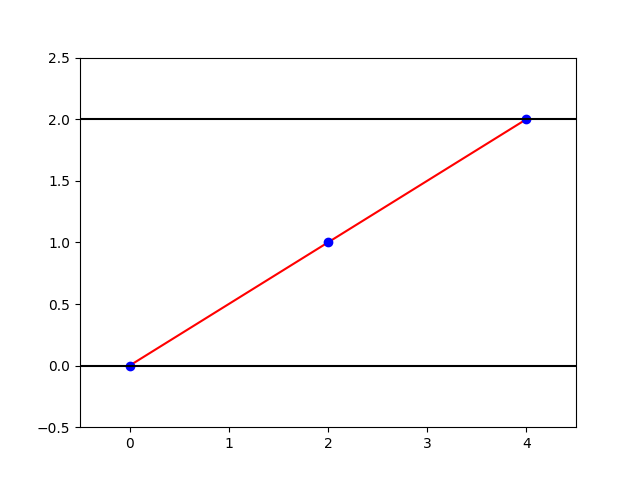
\includegraphics[width=0.75\textwidth]{hw4_figure_5}
		\centering
		\label{fig:p5a}
	\end{figure}
	In figure \ref{fig:p5a}, the interpolating polynomial is in red, the sample points are in blue, and the train tracks are in black.
	
%***************************************************************************************************
\problem{5 (b)} Adding the constraints that $f^\prime(0) = 0 = f^\prime(4)$ we calculate the divided difference

	\begin{center}
		\begin{tabular}{|c|c|c|c|c|c|}\hline
			$x_i$ & $f(x_i)$ & $f[x_{i-1},x_i]$ & $f[x_{x-2}, x_{i-1}, x_i]$ & $f[ x_{i-3}x_{i-2}, x_{i-1}, x_i]$ & $f[ x_{i-4},\dots, x_i]$ \\ \hline
			0 &0 & & & & \\ \hline
			0 &0 & 0 & & & \\ \hline
			2 &1 & $\tfrac{1}{2}$ & $\tfrac{1}{4}$ & & \\ \hline
			4 &2 & $\tfrac{1}{2}$ & 0 & $-\tfrac{1}{16}$ & \\ \hline
			4 &2 & 0 &  $-\tfrac{1}{4}$ & $-\tfrac{1}{16}$ & 0 \\ \hline
		\end{tabular}
	\end{center}

	Then our polynomial becomes
	$$
	P_4(x) = \tfrac{1}{4}(x-0)^2 - \tfrac{1}{16}(x-0)^2(x-2)
	$$

	\begin{figure}[H]
		\caption{The interpolating polynomial with zero slope at the end points}
		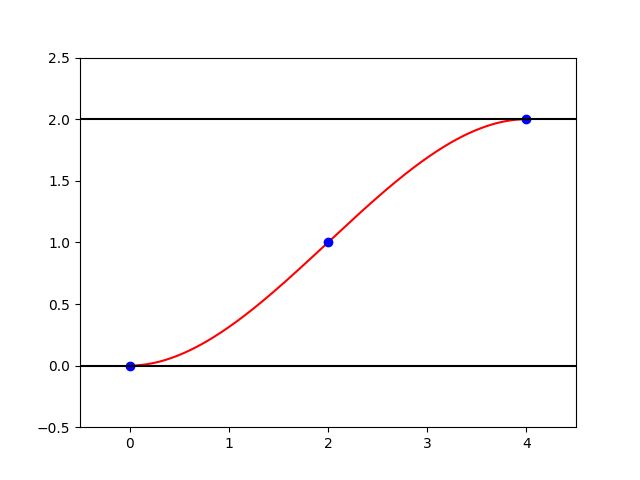
\includegraphics[width=0.75\textwidth]{hw4_figure_6}
		\centering
		\label{fig:p5b}
	\end{figure}
	In figure \ref{fig:p5b}, the interpolating polynomial is in red, the sample points are in blue, and the train tracks are in black. \bigbreak
	
%***************************************************************************************************
\problem{6(c)} Using the same constraints we can also fit two piecwise polynomials that meet at $(2,1)$ and each haveing slope $1$.

	
	

%***************************************************************************************************
\problem{6(a)} Show that the Chebyshev polynomials $T_n(x)=\cos{(n \arccos{x})}$ satisfy the following properties \\
\emph{(i)} $T_n(1) = 1$ \\
\emph{(ii)} $T_n(-1) = (-1)^n$ \\
\emph{(iii)} $T_j(x)T_k(x) = \tfrac{1}{2}[T_{j+k}(x) + T_{j-k}(x)]$ for $j>k\leq 0$. \\
\emph{(iv)} $\frac{T_{n+1}^\prime(x)}{n+1} - \frac{T_{n-1}^\prime(x)}{n-1} = 2T_n(x)$ for $n=1, 2, ...$ \\

	\begin{proof}
		Clearly $T_n(1) = \cos{(n \arccos{1})} = \cos{(n*0)} = \cos{(0)} = 1$, and thus we have (\emph{i}). \\
		
		In a similar fashion $T_n(-1) = \cos{(n \arccos{-1})} = \cos(n\pi)$ If $n$ is even $T_n(-1) = 1$ and if $n$ is odd then $T_n(-1)=-1$. This is also the case for $(-1)^n$. Thus $T_n(-1) = (-1)^n$ and we have (\emph{ii}). \\
		
		Recall the trig identity $cos(x)cos(y) = \tfrac{1}{2}[cos(x+y) + cos(x-y)]$, which will be useful in proving (\emph{iii}). Then
		\begin{align*}
			T_j(x)T_k(x) & = \cos(j \arccos{x}) \cos(k \arccos{x}) \\
			& = \tfrac{1}{2}[ \cos(j \arccos{x} + k \arccos{x}) +  \cos(j \arccos{x} k - k \arccos{x}) ] \\
			& = \tfrac{1}{2}[ \cos( (j + k) \arccos{x}) + \cos( (j - k) \arccos{x}) ]\\
			& = \tfrac{1}{2}[ T_{j+k}(x) + T_{j-k}(x)]
		\end{align*}
		Thus we have (\emph{iii}). \bigbreak
		
		For (\emph{iv}) it will be useful to recall that $\sin(x+y) - \sin(x-y) = 2 \cos(x) \sin(y)$ and that $\sin(\arccos(x)) = \sqrt{1-x^2}$. Also note that $T_n^\prime = -\sin{(n \arccos{x})} (-n)(1-x^2)^{-\frac{1}{2}}$. Then
		\begin{align*}
			\frac{T_{n+1}^\prime}{n+1} - \frac{T_{n-1}^\prime}{n-1} & = \frac{(n+1) \sin\big((n+1) \arccos(x) \big)}{(n+1)\sqrt{1-x^2}} - \frac{(n-1) \sin\big((n-1) \arccos(x) \big)}{(n-1)\sqrt{1-x^2}} \\
			& = \frac{ \sin\big((n+1) \arccos(x) \big) - \sin\big((n-1) \arccos(x) \big) } { \sqrt{1-x^2} } \\
			& =  \frac{2 \cos(n \arccos(x)) \sin(\arccos(x))}{ \sin(\arccos(x))} \\
			& = 2 T_n(x)
		\end{align*}
		Thus we have (\emph{iv}).		
	\end{proof}

%***************************************************************************************************
\problem{6 (b)} Prove that the Chebyshev polynomials are solutions to the differential equation
	
	\begin{align}\label{p1eq2}
	(1-x^2)y^{\prime\prime}-xy^\prime+n^2y=0
	\end{align}
	
	\begin{proof}
		Note that if $y = T_n(x)$, then
		\begin{align*}
		y^\prime & = -\sin{(n \arccos{x})} \tfrac{d}{dx}(n \arccos{x}) \\
		& = -\sin{(n \arccos{x})} (-n)(1-x^2)^{-\frac{1}{2}} \\
		& = n(1-x^2)^{-\frac{1}{2}}\sin{(n \arccos{x})}  \\
		y^{\prime\prime} &= -\tfrac{n}{2}(1-x^2)^{-\frac{3}{2}}(-2x)\sin{(n \arccos{x})} + n(1-x^2)^{-\frac{1}{2}}\cos{(n \arccos{x})}(-n)(1-x^2)^{-\frac{1}{2}} \\
		&= nx(1-x^2)^{-\frac{3}{2}}\sin{(n \arccos{x})} - n^2(1-x^2)^{-1}\cos{(n\arccos{x})}
		\end{align*}
		Then 
		\begin{align*}
		(1-x^2)y^{\prime\prime} & = (1-x^2) \Big( nx(1-x^2)^{-\frac{3}{2}}\sin{(n \arccos{x})} - n^2(1-x^2)^{-1}\cos{(n\arccos{x})} \Big) \\
		& = nx(1-x^2)^{-\frac{1}{2}}\sin{(n \arccos{x})} - n^2\cos{(n\arccos{x})} \\
		-xy^\prime & = -x n(1-x^2)^{-\frac{1}{2}}\sin{(n \arccos{x})} \\
		n^2y & = n^2\cos{(n \arccos{x})}
		\end{align*}
		Clearly these terms sum to zero and we have our result $(1-x^2)y^{\prime\prime}-xy^\prime+n^2y=0$. Thus $T_n$ are solutions to (\ref{p1eq2}).
		
	\end{proof}

%***************************************************************************************************
\singlespacing
\problem{7}

%***************************************************************************************************
\singlespacing
\problem{8}
	

\end{document}
